\chapter{Planificación temporal}
\label{ch:planificacion_temporal}

De cara a la realización de una planificación temporal se ha determinado un calendario de trabajo para el equipo de desarrollo implicado, en el proyecto que nos ocupa este equipo cuenta únicamente con un desarrollador. El desarrollador estará empleado en un trabajo ajeno al proyecto a jornada completa durante todo el transcurso del mismo. Los horarios serán diseñados en torno a dicha situación. El calendario resultante es el siguiente:

\vspace{-5pt}
\begin{itemize}
    \item Lunes a viernes: de 19:00 a 20:00
    \item Sábados: de 10:00 a 14:00
    \item Domingos: de 10:00 a 13:00
\end{itemize}

En total se establecerá un horario de trabajo semanal de 12 horas. Los descansos necesarios son incluidos en dichas jornadas. No se tendrán en cuenta festivos pero sí habrá días de parones por exceso de horas de trabajo acumuladas entre proyecto y empleo del desarrollador. Tanto la formación necesaria para el desarrollo del sistema como el tiempo dedicado al desarrollo de pruebas estará incluida en el tiempo de implementación de la características relacionadas, pues son labores paralelas al desarrollo de las mismas.

El inicio de desarrollo del proyecto ha sido establecido en el día de \textbf{1 de mayo de 2021}. Su finalización estimada tras el cálculo estimado será el día \textbf{15 de enero de 2022}. En resumen, el equipo de desarrollo se espera que dedique un máximo de doce horas semanales a lo largo de treinta y cinco semanas. La planificación temporal global es la ilustrada en el \fref{pt:general}, una más detallada se puede encontrar en los cuadros posteriores.

%{ p{0.1\textwidth} p{0.5\textwidth} p{0.15\textwidth} p{0.15\textwidth} }
\begin{longtable}{ c l c c c }
    \hline
    Código & Hito & Duración (h) & Predecesores & Desglose \\
    \hline
    1 & Arranque del proyecto & 7 & & \ref{pt:arranque_proyecto} \\
    2 & Planificación & 31 & 1 & \ref{pt:planificacion} \\
    3 & Análisis & 36 & 2 & \ref{pt:analisis} \\
    4 & Diseño & 46 & 3 & \ref{pt:diseño} \\
    5 & Implementación & 278 & 4 & \ref{pt:implementacion} \\
    6 & Elaboración de manuales & 9 & & \ref{pt:manuales} \\
    7 & Clausura del proyecto & 13 & 5, 6 & \ref{pt:clausura} \\
    \hline
    \caption{Planificación temporal global}
    \label{pt:general}
\end{longtable}

% Arranque
\begin{longtable}{ c p{0.5\textwidth} c c }
    \hline
    Código & Tarea & Duración (h) & Predecesoras \\
    \hline
    1 & \emph{Arranque del proyecto} & 7 & \\
    1.1 & Justificación & 2 & \\
    1.2 & Objetivos & 1 & \\
    1.3 & Estudio de la situación actual & 4 & \\
    \hline
    \caption{Planificación temporal del arranque de proyecto}
    \label{pt:arranque_proyecto}
\end{longtable}

% Planificación
\begin{longtable}{ c p{0.5\textwidth} c c }
    \hline
    Código & Tarea & Duración (h) & Predecesoras \\
    \hline
    2 & \emph{Planificación} & 31 & 1 \\
    2.1 & Requisitos iniciales & 2 &  \\
    2.2 & Evaluación de alternativas & 8 & 2.1 \\
    2.3 & Definición de la solución & 3 & 2.2 \\
    2.4 & Planificación temporal & 8 & 2.3 \\
    2.5 & Elaboración de presupuesto & 10 & 2.4 \\
    \hline
    \caption{Planificación temporal de la planificación del proyecto}
    \label{pt:planificacion}
\end{longtable}

% Análisis
\begin{longtable}{ c p{0.5\textwidth} c c }
    \hline
    Código & Tarea & Duración (h) & Predecesoras \\
    \hline
    3 & \emph{Análisis} & 36 & 2 \\
    3.1 & Identificación de requisitos & 12 &  \\
    3.2 & Identificación de subsistemas & 4 &  \\
    3.3 & Especificación de casos de uso & 5 &  \\
    3.4 & Bocetado de interfaces de usuario & 4 & 3.3 \\
    3.6 & Propuesta de clases del sistema & 8 & 3.1, 3.2, 3.4 \\
    3.7 & Especificación del plan de pruebas & 1 & 3.2 \\
    3.8 & Definición de plan de despliegue & 2 & 3.2 \\
    \hline
    \caption{Planificación temporal del análisis del sistema}
    \label{pt:analisis}
\end{longtable}

% Diseño
\begin{figure}[H]
\begin{longtable}{ c p{0.5\textwidth} c c }
    \hline
    Código & Tarea & Duración (h) & Predecesoras \\
    \hline
    4 & \emph{Diseño} & 46 & 3 \\
    4.1 & Definición de la arquitectura & 10 &  \\
    4.2 & Diseño de clases & 20 & 4.2 \\
    4.3 & Especificación del modelo de datos & 2 & 4.3 \\
    4.4 & Especificación de las interfaces de comunicación & 4 & 4.4 \\
    4.5 & Diseño de interfaces de usuario & 10 & 4.4 \\
    \hline
    \caption{Planificación temporal del diseño del sistema}
    \label{pt:diseño}
\end{longtable}
\end{figure}

% Implementación
\begin{longtable}{ c p{0.5\textwidth} c c }
    \hline
    Código & Tarea & Duración (h) & Predecesoras \\
    \hline
    5 & \emph{Implementación} & 278 & 4 \\
    5.1 & Prototipado & 6 &  \\
    5.2 & REST API & 53 & \\
    5.2.1 & \hspace{3mm}Autenticación & 6 & \\
    5.2.2 & \hspace{3mm}Usuarios & 15 & 5.2.1 \\
    5.2.3 & \hspace{3mm}Feed & 22 & 5.2.2 \\
    5.2.4 & \hspace{3mm}Tareas & 10 & 5.2.2 \\
    5.3 & WebSocket API & 39 & \\
    5.3.1 & \hspace{3mm}Global & 8 & 5.2.1 \\
    5.3.2 & \hspace{3mm}Mensajería & 17 & 5.2.3, 5.2.4 \\
    5.3.3 & \hspace{3mm}Localización & 2 & 5.2.1 \\
    5.3.4 & \hspace{3mm}Notificación & 12 & 5.2.3 \\
    5.4 & Despliegue del servidor & 14 & 5.2, 5.3 \\
    5.5 & Aplicación móvil & 166 &  \\
    5.5.1 & \hspace{3mm}Inicio y cierre de sesión & 11 & 5.2.1 \\
    5.5.2 & \hspace{3mm}Pantalla principal & 9 & 5.5.1 \\
    5.5.3 & \hspace{3mm}Vinculación & 20 & 5.22 \\
    5.5.4 & \hspace{3mm}Listado de vínculos & 15 & 5.22 \\
    5.5.5 & \hspace{3mm}Geolocalización & 29 & 5.3.3 \\
    5.5.6 & \hspace{3mm}Feed & 37 & 5.2.3, 5.2.4, 5.3.2 \\
    5.5.7 & \hspace{3mm}Gestión de tareas & 25 & 5.2.4 \\
    5.5.8 & \hspace{3mm}Notificaciones & 20 & 5.2.3, 5.3.4 \\
    \hline
    \caption{Planificación temporal de la implementación del sistema}
    \label{pt:implementacion}
\end{longtable}

% Manuales
\begin{longtable}{ c p{0.5\textwidth} c c }
    \hline
    Código & Tarea & Duración (h) & Predecesoras \\
    \hline
    6 & \emph{Elaboración de manuales} & 9 & \\
    6.1 & Manual de usuario & 4 & 5.5 \\
    6.2 & Manual de instalación & 1 & 5.5 \\
    6.3 & Manual de despliegue & 2 & 5.4 \\
    6.4 & Manual de desarrollador & 2 & 5 \\
    \hline
    \caption{Planificación temporal de la elaboración de manuales}
    \label{pt:manuales}
\end{longtable}

% Clausura
\begin{longtable}{ c p{0.5\textwidth} c c }
    \hline
    Código & Tarea & Duración (h) & Predecesoras \\
    \hline
    7 & \emph{Clausura del proyecto} & 13 & 6 \\
    7.1 & Redacción de conclusiones & 2 &  \\
    7.2 & Definición de ampliaciones & 2 &  \\
    7.3 & Revisión de conclusión & 9 & 7.1, 7.2 \\
    \hline
    \caption{Planificación temporal de la clausura del proyecto}
    \label{pt:clausura}
\end{longtable}

\begin{sidewaysfigure}
    \centering
    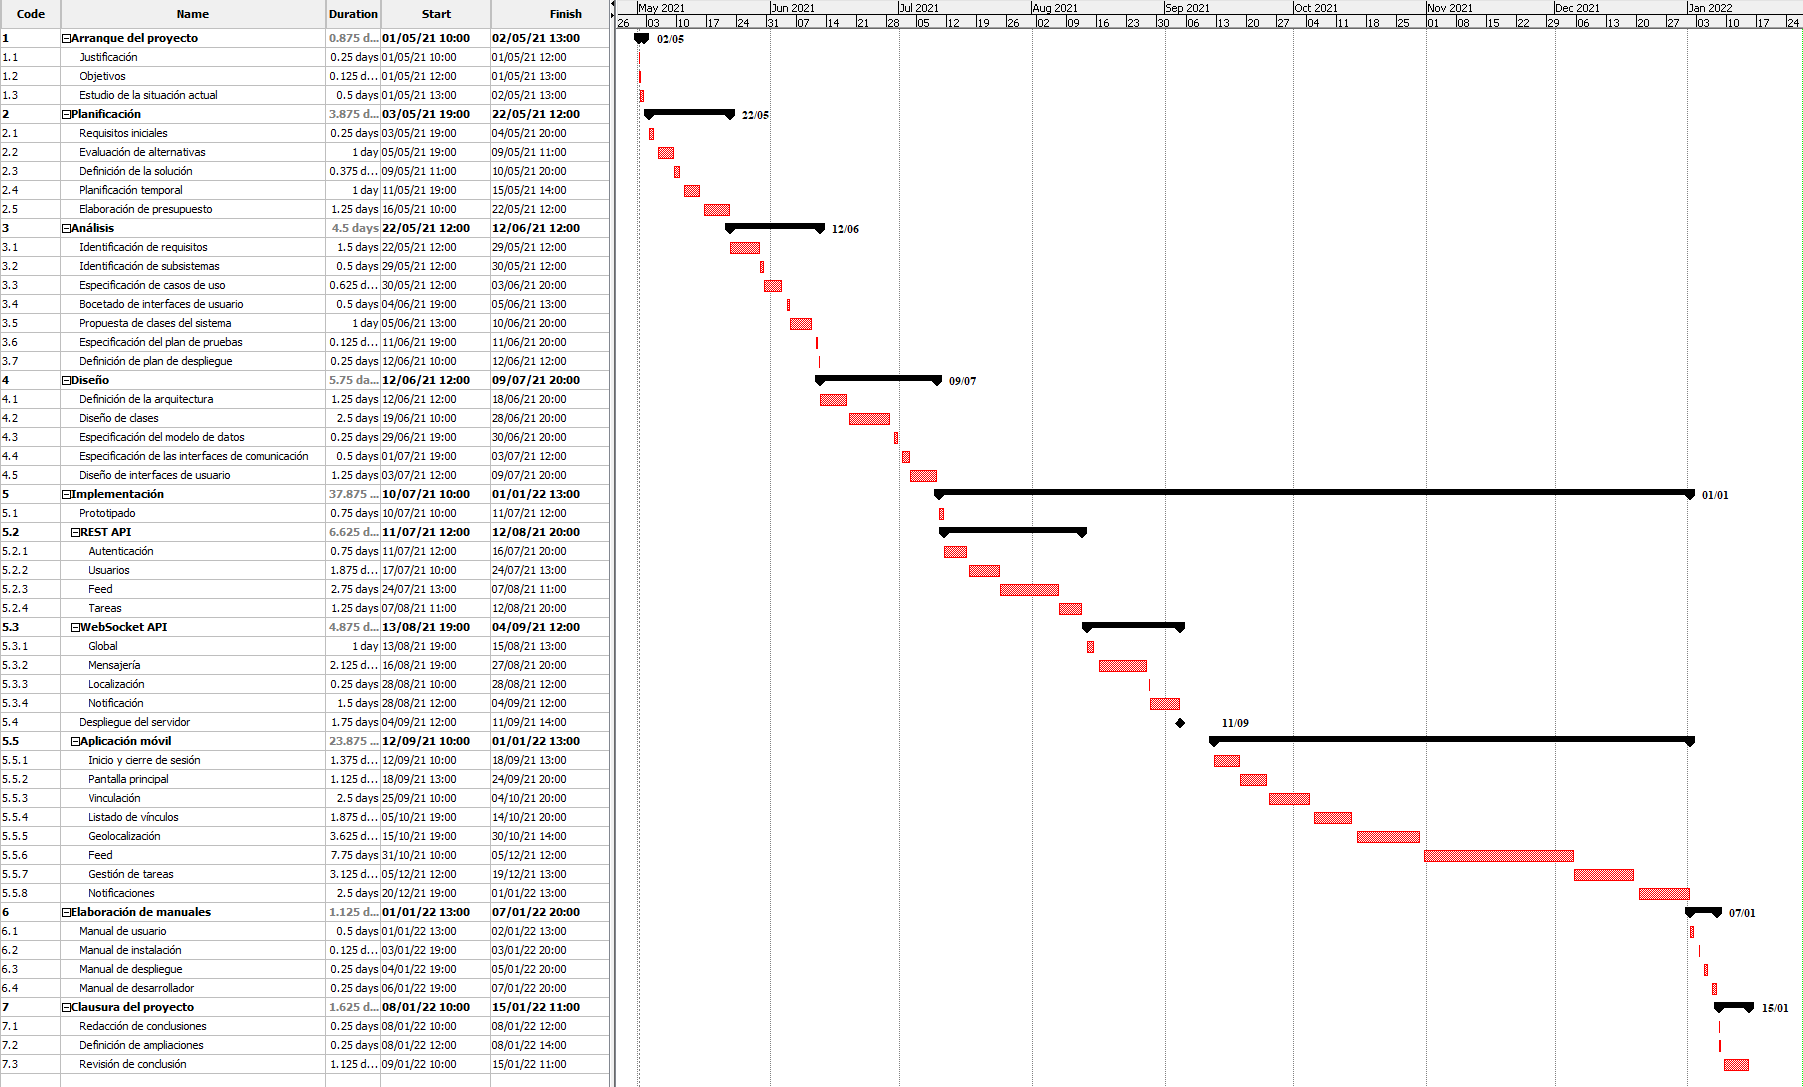
\includegraphics[width=1\textwidth]{images/Anexos/DiagramaGantt.png}
    \caption{Diagrama de Gantt del proyecto}
    \label{dia:gantt}
\end{sidewaysfigure}